\section{Evaluation}
\label{sec:eval}

\subsection{Experimental Setting}
\label{sec:expSet}

\begin{table}[t]
%\small
\caption{\label{tab:data} TREC collections used for experiments.}
\begin{tabular}{@{}lll@{}}
& \robust & \cw \\
\toprule
Data & Disks $4$ \& $5$ (-CR) & ClueWeb12 Category B \\
Documents & 528,155 & 52,343,021 \\
Topics & $301$-$450$, $600$-$700$ & $201$-$300$ \\
Average number of   & $12.5$ $$ & $45.4$ \\
queries per topic
\end{tabular}

\end{table}


\myparagraph{Data} We use two TREC collections for experiments:
\robust, a small collection of mainly news documents and \cw, a much
larger collection of Web pages. Each collection is associated with a
set of TREC topics portraying different information needs. In prior
work on cluster-based retrieval, a single query served for
representing a topic. This query, henceforth \emph{title query}, was
typically the topic's title.  In this work, in addition to the title
query, we use queries which were written by crowd workers to represent
the same topic~\cite{bailey2016uqv100,bc17-adcs}.\footnote{The queries
  are publicly available at \url{https://tinyurl.com/robustuqv} and
  \url{https://tinyurl.com/clue12uqv}.} Recent work shows the
performance similarities between these human-generated queries and
reformulations automatically selected from a search engine's query log \cite{Liu+al:19a}.
Further details about the
document collections, topics and queries are provided in
Table~\ref{tab:data}.\footnote{Topic $672$ for \robust was discarded
  as none of the judged documents for this topic was relevant.}


All queries and documents were stemmed using the Krovetz stemmer. Stopwords on the INQUERY list were removed from queries. We discarded duplicate queries and queries with out-of-vocabulary terms. Our experiments were performed using the Indri toolkit.\footnote{\url{www.lemurproject.org/indri}} 

The set of queries $\querySet$ per TREC topic consists of the title
query and $\numQuery$ {\em additional} queries randomly sampled from
all those available for the topic. To prevent potential sampling bias,
we repeat the experiments $30$ times by using $30$ random samples of query sets; we
then report the average performance over the samples.

\myparagraph{Evaluation metrics}
To study the extent to which the cluster hypothesis holds for a document set $\arbSet$, we apply Voorhees' nearest-neighbor test~\cite{Voorhees:85a}. 
For each relevant document $\doc \in \arbSet$, we count the number of relevant documents among its $\clustSize-1$ nearest neighbors, i.e., the $\clustSize-1$ documents $\doc' \in \arbSet$ ($\doc' \ne \doc$) that yield the highest $\simFn{\doc}{\doc'}$. The average of these counts is divided by the total number of relevant documents in $\arbSet$. The test is performed for TREC topics with $|\arbSet| > 1$ and the result reported is the average across these topics.


To evaluate retrieval performance, we use \map: Mean Average Precision of the top-$\numRet$ documents, \precFive: precision of the top-$5$ documents, and \ndcg: Normalized Discounted Cumulative Gain of the top-$20$ documents. Recall that the cluster-based methods in all the templates re-rank lists of $\numRet$ documents. Statistically significant differences of performance are computed using the two-tailed paired t-test at a $95\%$ confidence level with Bonferroni correction for multiple testing.



\myparagraph{Baselines}
%We compare the performance of our proposed approaches with the query expansion method \ariRM~\cite{Lu+al:19a}. As in our setting, \ariRM assumes that multiple queries representing the same information need are available for retrieval. \ariRM makes use of the queries by fusing the relevance models induced from these queries~\cite{Lavrenko+Croft:01a}.
We compare the performance of our proposed templates when instantiated
with different cluster-based retrieval methods with the performance
of these methods when a single title query is used which is the standard
practice.

We also use for reference the effectiveness of the
different document lists upon which the cluster-based templates are
applied.  For \queryCat, the document list is retrieved in response to
the concatenated query $\conQuery$. For \fuseClust, the document list is created
by fusing the multiple initial lists retrieved in response to each of
the queries in $\querySet$. As already noted, we use the
reciprocal-rank fusion (RRF) method~\cite{Cormack+al:09a} that was shown to
be highly effective in fusing lists retrieved in response to multiple queries representing the same information need~\cite{bailey2017retrieval,bc17-adcs}. For \feature, we use
the cluster-based templates upon the list of documents
retrieved with respect to the title query.  Note that the initial
lists used in the \poolClust and \clustFuse templates cannot serve as
baselines: in \poolClust the cluster-based methods are applied to an
unordered list of documents and in \clustFuse the methods are applied
to multiple lists.

An additional baseline is the query expansion method \ariRM
which utilizes multiple queries representing the same information need
~\cite{Lu+al:19a}. \ariRM constructs a single relevance model by fusing the relevance models induced from the lists retrieved in response to the queries. 

%As in our setting, \ariRM assumes that multiple
%queries representing the same information need are available for
%retrieval. \ariRM makes use of the queries by fusing the relevance
%models induced from these queries~\cite{Lavrenko+Croft:01a}.


\myparagraph{Feature weights, free-parameter values and additional implementation details}
To set the free-parameter values of all methods, and to learn feature weights in \clustMRF, we used cross validation over topics. The topics were divided into five folds based on their IDs. One fold was retained for testing in a round-robin fashion. For all the methods except for \clustMRF, free-parameter values were selected based on the four remaining training folds. For \clustMRF~\cite{Raiber+Kurland:13a}, three out of the four folds were used to learn feature weights for each configuration of the free-parameter values. The learned models were applied to the fourth fold that served for validation. This procedure was repeated four times where each time a different fold was held out for validation. The free-parameter values were selected based on the average performance over the topics in the four validation folds. A final model was then learned using all four training folds. The feature weights in \clustMRF were learned using linear SVM$^{rank}$\footnote{\url{www.svmlight.joachims.org}} applied with default hyper-parameter values. We report in all cases the average performance over all the topics per dataset when these were part of the test folds. \map served for the optimization metric in all the experiments.

Cluster-based document retrieval methods were shown to perform particularly well when applied upon relatively short document lists~\cite{Raiber+Kurland:13a}. Accordingly, we set the number of documents in the initial lists, $\numRet$, to $100$.\footnote{Experiments with setting $\numRet=50$ resulted in relative performance patterns highly similar to those for $\numRet=100$. The actual numbers are omitted as they convey no additional insight.} The size of the nearest-neighbor clusters $\clustSize$ was selected from $\set{5,10}$ as in past work~\cite{Kurland+Domshlak:08a,Kurland:09a,Kurland+Krikon:11a,Raiber+Kurland:13a}. The Dirichlet smoothing parameter $\dirParam$ for inducing language models (Section~\ref{sec:retAlg}) is set to $1000$~\cite{Zhai+Lafferty:01a}.
We experimented with different values of $\numQuery$, the number of sampled queries in $\querySet$: $\set{1,3,5,10}$ queries were used for \robust and $\set{1,5,15,25}$ for \cw~\cite{Lu+al:19a}.
The value of $\alpha$ in the reciprocal-rank fusion method was selected from $\set{30,60,90}$. The value of $ \lambda$ in \interp is in $\set{0,0.1,\ldots,1}$.
We clipped the concatenated query $\conQuery$ in \queryCat to the $\set{5,10,25,All}$\footnote{``$All$'' means that no clipping was applied.} terms assigned with the highest probabilities by the unsmoothed maximum likelihood estimate induced from $\conQuery$. (Refer back to Section~\ref{sec:retAlg} for details.)

We used the title query to represent the query set $\querySet$ in \feature; that is, the cluster-based methods in \feature were applied to the top-$\numRet$ document retrieved in response to the title query by the document-based method.
Note that this approach is similar to the standard practice of using a single (title) query with the difference that additional evidence from other queries is incorporated at the feature level.
%The baseline method, \ariRM, was also applied to this list.
The baseline method, \ariRM, was applied upon the list
$\retList_{fuse}$ as in the \fuseClust template.\footnote{Applying
  \ariRM on the initial document list retrieved with respect to the
  title query resulted in less effective performance. Some recent work demonstrated the merits of using relevance models for re-ranking in comparison to ranking the entire corpus \cite{Diaz:15a}. Here, the relevance model of \ariRM is used to re-rank a highly effective document list attained by using RRF to fuse the initially retrieved lists.}  The number of
top-ranked documents used to induce the relevance models in \ariRM was
selected from $\set{25,50}$; the term-clipping ($\beta$) and
query-anchoring ($\lambda$) parameters were set to values in
$\set{5,10,25,50}$ and $\set{0,0.1,\ldots,1}$, respectively.


\subsection{Experimental Results}
\label{sec:results}

\subsubsection{Query effectiveness}
Previous research has shown that standard language-model-based document retrieval performance can vary considerably depending on the query used to represent the information need~\cite{Lu+al:19a,Zendel+al:19a}. Researchers have also shown that query-performance prediction quality can be substantially affected by the effectiveness of the query~\cite{Zendel+al:19a}. In what follows, we examine the impact of the query used on the performance of existing cluster-based retrieval methods, the results of the cluster hypothesis test and the percentage of relevant documents in the optimal cluster. 

We assume in these experiments that only one query, not necessarily the title query, is available for retrieval per topic. To select the representing query, we divided all the queries of a topic into quartiles based on the effectiveness (determined using Average Precision; AP@$\numRet$) of the initial lists (\init) that were retrieved in response to these queries and upon which the cluster-based retrieval methods operate. We consider the first (\qOneAP), second (\medAP) and third (\qThreeAP) quartile queries as representatives. We also consider the best performing query (\maxAP) and the title (\titleQuery) query. The latter deserves special attention as it was used to represent topics in past research on cluster-based retrieval.


\begin{table*}[t]
%\tabcolsep=0.05cm
%\small
\caption{\label{tab:variance}The effectiveness of the initial ranking and the \emph{percentage} of relative change in the performance of cluster-based retrieval methods with respect to the initial ranking when queries of varying effectiveness are used to represent topics. `$\statSymbolInit$' marks statistically significant differences with \init. The highest percentages per row and collection are underlined.}
\begin{tabular}{@{}llrrrrrrrrrrr@{}}
& &
\multicolumn{5}{c}{\robust} & \multicolumn{5}{c}{\cw}\\
\cmidrule(r){3-7} \cmidrule(l){8-12}
& & \titleQuery & \qOneAP\initSpace\initSpace  & \medAP\initSpace\initSpace & \qThreeAP\initSpace\initSpace&\maxAP\initSpace & \titleQuery & \qOneAP  & \medAP\initSpace\initSpace & \qThreeAP\initSpace\initSpace &\maxAP\initSpace\initSpace \\
\toprule
\multirow{3}{*}{\init } & \map & $.216\initSpace$ & $.154\initSpace$ & $.199\initSpace$ & $.249\initSpace$ & $.342\initSpace$ & $.148\initSpace$ & $.081$ & $.123\initSpace$ & $.160\initSpace$ & $.222\initSpace$\\
& \precFive & $.487\initSpace$ & $.383\initSpace$ & $.448\initSpace$ & $.562\initSpace$ & $.700\initSpace$ & $.444\initSpace$ & $.388$ & $.482\initSpace$ & $.538\initSpace$ & $.718\initSpace$\\
& \ndcg & $.410\initSpace$ & $.305\initSpace$ & $.377\initSpace$ & $.461\initSpace$ & $.578\initSpace$ & $.415\initSpace$ & $.321$ & $.417\initSpace$ & $.484\initSpace$ & $.631\initSpace$\\
\addlinespace
\multirow{3}{*}{\clustMRF } & \diffp{\map} & $6.5^{\statSymbolInit}$ & $\underline{10.4}^{\statSymbolInit}$ & $5.3^{\statSymbolInit}$ & $5.1^{\statSymbolInit}$ & $-2.4^{\statSymbolInit}$ & $-3.3^{\statSymbolInit}$ & $\underline{5.5}$ & $2.0\initSpace$ & $0.0\initSpace$ & $-6.5^{\statSymbolInit}$\\
& \diffp{\precFive} & $5.0^{\statSymbolInit}$ & $\underline{6.9}^{\statSymbolInit}$ & $5.2\initSpace$ & $2.9\initSpace$ & $-1.7\initSpace$ & $-1.8\initSpace$ & $3.1$ & $4.6\initSpace$ & $\underline{7.8}^{\statSymbolInit}$ & $-3.6\initSpace$\\
& \diffp{\ndcg} & $3.4^{\statSymbolInit}$ & $\underline{8.3}^{\statSymbolInit}$ & $4.1^{\statSymbolInit}$ & $3.8^{\statSymbolInit}$ & $-2.3^{\statSymbolInit}$ & $-2.1\initSpace$ & $-0.8$ & $\underline{2.8}\initSpace$ & $2.2\initSpace$ & $-6.6^{\statSymbolInit}$\\
\addlinespace
\multirow{3}{*}{\geoClust } & \diffp{\map} & $6.4^{\statSymbolInit}$ & $9.5^{\statSymbolInit}$ & $\underline{9.8}^{\statSymbolInit}$ & $8.6^{\statSymbolInit}$ & $-0.8\initSpace$ & $-3.8^{\statSymbolInit}$ & $\underline{4.3}$ & $-0.6\initSpace$ & $1.7\initSpace$ & $-4.4^{\statSymbolInit}$\\
& \diffp{\precFive} & $0.8\initSpace$ & $0.0\initSpace$ & $\underline{9.9}^{\statSymbolInit}$ & $6.6^{\statSymbolInit}$ & $-3.2^{\statSymbolInit}$ & $-5.0\initSpace$ & $0.0$ & $-2.9\initSpace$ & $\underline{1.5}\initSpace$ & $1.1\initSpace$\\
& \diffp{\ndcg} & $1.9\initSpace$ & $7.2^{\statSymbolInit}$ & $\underline{7.9}^{\statSymbolInit}$ & $7.0^{\statSymbolInit}$ & $-1.0\initSpace$ & $-4.0^{\statSymbolInit}$ & $-3.0$ & $-4.9^{\statSymbolInit}$ & $\underline{1.2}\initSpace$ & $-5.6^{\statSymbolInit}$\\
\addlinespace
\multirow{3}{*}{\interp } & \diffp{\map} & $3.5^{\statSymbolInit}$ & $6.7^{\statSymbolInit}$ & $\underline{6.8}^{\statSymbolInit}$ & $4.8^{\statSymbolInit}$ & $1.7^{\statSymbolInit}$ & $\underline{0.0}\initSpace$ & $\underline{0.0}$ & $\underline{0.0}\initSpace$ & $-0.2\initSpace$ & $\underline{0.0}\initSpace$\\
& \diffp{\precFive} & $1.2\initSpace$ & $1.7\initSpace$ & $\underline{9.9}^{\statSymbolInit}$ & $3.4^{\statSymbolInit}$ & $1.9^{\statSymbolInit}$ & $0.0\initSpace$ & $0.0$ & $0.0\initSpace$ & $\underline{1.1}^{\statSymbolInit}$ & $0.0\initSpace$\\
& \diffp{\ndcg} & $2.0\initSpace$ & $3.5^{\statSymbolInit}$ & $\underline{8.2}^{\statSymbolInit}$ & $4.9^{\statSymbolInit}$ & $1.8^{\statSymbolInit}$ & $0.0\initSpace$ & $0.0$ & $0.0\initSpace$ & $\underline{0.1}\initSpace$ & $0.0\initSpace$\\

\end{tabular}

\end{table*}

\myparagraph{Cluster-based retrieval}
Table~\ref{tab:variance} presents the effectiveness  (\map, \precFive and \ndcg) of the initial rankings (\init) created in response to each of the queries and the percentage of relative change in performance (\diffp{\map}, \diffp{\precFive} and \diffp{\ndcg}) of the cluster-based retrieval methods (\clustMRF, \geoClust and \interp) with respect to \init.
Our first observation is that the majority of the numbers reported in the table are positive. This indicates that applying cluster-based retrieval often results in improved performance regardless of the effectiveness of the queries used; many of the improvements are statistically significant, especially for the \robust collection. The main exception is for highly effective queries (\maxAP) which we discuss below. 

% are a few cases where performance is impaired (negative numbers) and in only a few of these cases the differences are statistically significant. This finding attests to the fact that cluster-based document retrieval methods are highly effective not only for the title query but also for other queries of varying effectiveness.

We also see in Table~\ref{tab:variance} that \clustMRF is better than
\interp on \robust for \titleQuery and \qOneAP queries, while the
reverse holds for \medAP and \maxAP queries. On \cw, \clustMRF is
better than \geoClust for \titleQuery, \qOneAP and \medAP queries, but
the reverse holds for \qThreeAP and \maxAP. Thus, we arrive to the conclusion that the relative effectiveness of
different cluster-based document retrieval methods can change depending on the
effectiveness of the query used to represent the information need. This conclusion has far reaching implications given that previous work on cluster-based document retrieval (as most other work on document retrieval) used the \titleQuery queries for evaluation.
A similar conclusion was drawn about the
relative prediction quality of query-performance prediction
methods~\cite{Zendel+al:19a}. 

Another interesting observation that we make based on Table~\ref{tab:variance} is that the improvements in the performance of cluster-based retrieval methods tend to decrease for exceptionally effective queries.
That is, the improvements attained for \maxAP are often lower than those attained for \qOneAP, \medAP and \qThreeAP. In fact, in most cases, cluster-based retrieval does not improve performance over the initial document ranking.
A case in point, the state-of-the-art method \clustMRF can actually become less effective than the initial ranking for the most effective queries (e.g., \maxAP on \robust).
%The results for the \titleQuery query are quite different than those for the other representatives. For example, for \robust, the improvements for \titleQuery are in most cases the lowest among the considered queries whereas for \cw, there are no clear trends.


\myparagraph{Cluster hypothesis}
In Table~\ref{tab:clustHypo} we present the results of the cluster hypothesis test. The test is applied to the initial document lists retrieved with respect to the \titleQuery, \qOneAP, \medAP, \qThreeAP and \maxAP queries. We see that the hypothesis holds to a larger extent as the query representing the information need becomes less effective, e.g., contrast \qOneAP with \medAP, \medAP with \qThreeAP and \qThreeAP with \maxAP.  Most of the differences with \qOneAP, the least effective query which is also the one for which the hypothesis holds to the largest extent, are statistically significant. This finding, which is novel to our work, implies that documents retrieved with respect to poorly (highly) performing queries tend to be more (less) similar compared to those retrieved with respect to more (less) effective queries.
Moreover, this finding is directly related to the phenomenon we observed in Table~\ref{tab:variance} about cluster-based retrieval methods tending to be relatively less effective for highly performing queries.


\begin{table}[t]
%\small
\caption{\label{tab:clustHypo}The cluster hypothesis test. `$\statSymbolInit$' marks statistically significant differences with \qOneAP. Underline: highest result per collection.}
\begin{tabular}{@{}lccccc@{}}
& \titleQuery & \qOneAP & \medAP & \qThreeAP & \maxAP \\
\toprule
\robust & $.159\initSpace$ &  $\underline{.171}$ & $.166\initSpace$ & $.152^{\statSymbolInit}$ & $.137^{\statSymbolInit}$\\
\cw & $.080^{\statSymbolInit}$ & $\underline{.097}$ &  $.084^{\statSymbolInit}$ &  $.074^{\statSymbolInit}$ &  $.071^{\statSymbolInit}$ \\
\end{tabular}
\end{table}

\begin{table}[t]
%\small
\caption{\label{tab:optClust}The percentage of relevant documents in the optimal cluster. `$\statSymbolInit$' marks statistically significant differences with \maxAP. Underline: highest value per collection.}
\begin{tabular}{@{}lccccc@{}}
& \titleQuery & \qOneAP & \medAP & \qThreeAP & \maxAP \\
\toprule
\robust & $82.2^{\statSymbolInit}$ & $76.5^{\statSymbolInit}$ & $83.2^{\statSymbolInit}$ & $86.3^{\statSymbolInit}$ &$\underline{89.6}$\\
\cw & $80.2^{\statSymbolInit}$ & $74.6^{\statSymbolInit}$ & $82.0^{\statSymbolInit}$ & $85.2^{\statSymbolInit}$& $\underline{91.6}$ \\
\end{tabular}
\end{table}
\begin{table*}[t]
%\small
\caption{\label{tab:main} Main result. Comparing the two most effective methods instantiated from our templates, \inst{\clustMRF}{\clustFuse} and \inst{\interp}{\queryCat}, with the various baselines. $\numQuery=5$ and $\numQuery=15$ queries, in addition to the \titleQuery query, were used for ROBUST and CW12, respectively. Superscripts `$\statSymbolRRF$' - `$\statSymbolAriRMfuse$' indicate statistically significant differences (after Bonferroni correction) with respect to the numbered baselines. Underline: best result in a column.}
\begin{tabular}{lllllll}
&
\multicolumn{3}{c}{\robust} &
\multicolumn{3}{c}{\cw}\\
\cmidrule(r){2-4} \cmidrule(l){5-7}
\multirow{1}{*}{} &
\multicolumn{1}{c}{\map} &
\multicolumn{1}{c}{\precFive}&
\multicolumn{1}{c}{\ndcg} &
\multicolumn{1}{c}{\map} &
\multicolumn{1}{c}{\precFive}&
\multicolumn{1}{c}{\ndcg}  \\

\toprule
\textsuperscript{\statSymbolRRF}\inst{\init}{\fuseClust}
&
$.268$ &
$.593$ &
$.481$ &
$.197$ &
$.560$ &
$.512$ 
\\
\textsuperscript{\statSymbolQLtitle}\inst{\init}{\feature}
&
$.224\stackanchor{}{\statSymbolRRF}$ &
$.481\stackanchor{}{\statSymbolRRF}$ &
$.405\stackanchor{}{\statSymbolRRF}$ &
$.148\stackanchor{}{\statSymbolRRF}$ &
$.444\stackanchor{}{\statSymbolRRF}$ &
$.415\stackanchor{}{\statSymbolRRF}$ 
\\
\textsuperscript{\statSymbolQLconc}\inst{\init}{\queryCat}
&
$.288\stackanchor{}{\statSymbolRRF\statSymbolQLtitle}$ &
$.603\stackanchor{}{\statSymbolQLtitle}$ &
$.496\stackanchor{}{\statSymbolRRF\statSymbolQLtitle}$ &
$.157\stackanchor{}{\statSymbolRRF}$ &
$.511\stackanchor{}{\statSymbolRRF\statSymbolQLtitle}$ &
$.458\stackanchor{}{\statSymbolRRF\statSymbolQLtitle}$ 
\\
\textsuperscript{\statSymbolCMRFtitle}\inst{\clustMRF}{\titleQuery}
&
$.231\stackanchor{}{\statSymbolRRF\statSymbolQLconc}$ &
$.511\stackanchor{}{\statSymbolRRF\statSymbolQLconc}$ &
$.423\stackanchor{}{\statSymbolRRF\statSymbolQLconc}$ &
$.143\stackanchor{}{\statSymbolRRF\statSymbolQLconc}$ &
$.436\stackanchor{}{\statSymbolRRF\statSymbolQLconc}$ &
$.406\stackanchor{}{\statSymbolRRF\statSymbolQLconc}$ 
\\
\textsuperscript{\statSymbolGeoClustTitle}\inst{\geoClust}{\titleQuery}
&
$.230\stackanchor{}{\statSymbolRRF\statSymbolQLconc}$ &
$.491\stackanchor{}{\statSymbolRRF\statSymbolQLconc}$ &
$.417\stackanchor{}{\statSymbolRRF\statSymbolQLconc}$ &
$.142\stackanchor{}{\statSymbolRRF\statSymbolQLconc}$ &
$.422\stackanchor{}{\statSymbolRRF\statSymbolQLconc}$ &
$.398\stackanchor{}{\statSymbolRRF\statSymbolQLconc}$ 
\\
\textsuperscript{\statSymbolInterpTitle}\inst{\interp}{\titleQuery}
&
$.224\stackanchor{}{\statSymbolRRF\statSymbolQLconc}$ &
$.492\stackanchor{}{\statSymbolRRF\statSymbolQLconc}$ &
$.418\stackanchor{}{\statSymbolRRF\statSymbolQLtitle\statSymbolQLconc}$ &
$.148\stackanchor{}{\statSymbolRRF}$ &
$.444\stackanchor{}{\statSymbolRRF\statSymbolQLconc}$ &
$.415\stackanchor{}{\statSymbolRRF\statSymbolQLconc}$ 
\\
\textsuperscript{\statSymbolAriRMfuse}\ariRM
&
$.271\stackanchor{}{\statSymbolQLtitle\statSymbolQLconc\statSymbolCMRFtitle\statSymbolInterpTitle}$ &
$.576\stackanchor{}{\statSymbolQLtitle\statSymbolQLconc\statSymbolCMRFtitle\statSymbolInterpTitle}$ &
$.476\stackanchor{}{\statSymbolQLtitle\statSymbolQLconc\statSymbolCMRFtitle\statSymbolInterpTitle}$ &
$.188\stackanchor{}{\statSymbolRRF\statSymbolQLtitle\statSymbolQLconc\statSymbolCMRFtitle\statSymbolInterpTitle}$ &
$.507\stackanchor{}{\statSymbolRRF\statSymbolQLtitle\statSymbolInterpTitle}$ &
$.477\stackanchor{}{\statSymbolRRF\statSymbolQLtitle\statSymbolCMRFtitle\statSymbolInterpTitle}$ 
\\
\addlinespace
\midrule
\inst{\clustMRF}{\clustFuse}
&
$.280\stackanchor{}{\statSymbolRRF\statSymbolQLtitle\statSymbolCMRFtitle\statSymbolGeoClustTitle\statSymbolInterpTitle}$ &
$\underline{.608}\stackanchor{}{\statSymbolQLtitle\statSymbolCMRFtitle\statSymbolGeoClustTitle\statSymbolInterpTitle\statSymbolAriRMfuse}$ &
$.499\stackanchor{}{\statSymbolRRF\statSymbolQLtitle\statSymbolCMRFtitle\statSymbolGeoClustTitle\statSymbolInterpTitle\statSymbolAriRMfuse}$ &
$\underline{.210}\stackanchor{}{\statSymbolRRF\statSymbolQLtitle\statSymbolQLconc\statSymbolCMRFtitle\statSymbolGeoClustTitle\statSymbolInterpTitle\statSymbolAriRMfuse}$ &
$\underline{.640}\stackanchor{}{\statSymbolRRF\statSymbolQLtitle\statSymbolQLconc\statSymbolCMRFtitle\statSymbolGeoClustTitle\statSymbolInterpTitle\statSymbolAriRMfuse}$ &
$\underline{.566}\stackanchor{}{\statSymbolRRF\statSymbolQLtitle\statSymbolQLconc\statSymbolCMRFtitle\statSymbolGeoClustTitle\statSymbolInterpTitle\statSymbolAriRMfuse}$ 
\\
\inst{\interp}{\queryCat}
&
$\underline{.290}\stackanchor{}{\statSymbolRRF\statSymbolQLtitle\statSymbolCMRFtitle\statSymbolGeoClustTitle\statSymbolInterpTitle\statSymbolAriRMfuse}$ &
$\underline{.608}\stackanchor{}{\statSymbolRRF\statSymbolQLtitle\statSymbolCMRFtitle\statSymbolGeoClustTitle\statSymbolInterpTitle\statSymbolAriRMfuse}$ &
$\underline{.502}\stackanchor{}{\statSymbolRRF\statSymbolQLtitle\statSymbolQLconc\statSymbolCMRFtitle\statSymbolGeoClustTitle\statSymbolInterpTitle\statSymbolAriRMfuse}$ &
$.193\stackanchor{}{\statSymbolQLtitle\statSymbolQLconc\statSymbolCMRFtitle\statSymbolGeoClustTitle\statSymbolInterpTitle}$ &
$.577\stackanchor{}{\statSymbolQLtitle\statSymbolQLconc\statSymbolCMRFtitle\statSymbolGeoClustTitle\statSymbolInterpTitle\statSymbolAriRMfuse}$ &
$.522\stackanchor{}{\statSymbolQLtitle\statSymbolQLconc\statSymbolCMRFtitle\statSymbolGeoClustTitle\statSymbolInterpTitle\statSymbolAriRMfuse}$ 
\\


\end{tabular}
\end{table*}

\myparagraph{Optimal cluster}
%Table~\ref{tab:optClust} presents the percentage of relevant documents in the optimal cluster. The analysis is performed upon the initial document lists.
We next examine the optimal cluster phenomenon for queries of varying effectiveness. For a given set $\arbSet$ of documents per topic, we compute the percentage of relevant documents in each cluster $\clust \in \cluster{\arbSet}$. The maximum percentage is the topic's score. The final score is the average across the topics. Table~\ref{tab:optClust} presents the results for the initial document lists retrieved with respect to the different queries we consider.
We see that the percentages can vary greatly depending on the query used, e.g., from $74.6$ for \qOneAP to $91.6$ for \maxAP on CW12.  In general, the percentage of relevant documents in the optimal cluster increases with increase in query effectiveness. 


\subsubsection{Main results of the retrieval templates}



%\begin{table*}[t]
%\small
%\caption{\label{tab:mainTwo}Main results two?. Superscripts `$\statSymbolRRF$' - `$\statSymbolAriRMfuse$' indicate statistically significant% differences with respect to the numbered baselines. Bold: best result in a column.}
%\begin{tabular}{|l|l| l| l| l| l| l| l| l| l| l| l| l| l| l| l| l| l| l| l| l| l| l| l| l|}

\hline
\multirow{1}{*}{v} &
\multicolumn{3}{c|}{5} &
\multicolumn{3}{c|}{15}\\
\hline
\multirow{1}{*}{} &
\multicolumn{1}{c|}{MAP} &
\multicolumn{1}{c|}{P@5}&
\multicolumn{1}{c|}{NDCG} &
\multicolumn{1}{c|}{MAP} &
\multicolumn{1}{c|}{P@5}&
\multicolumn{1}{c|}{NDCG}  \\

\hline

\textsuperscript{1}RRF
&
$.268$ &
$.593$ &
$.481$ &
$.197$ &
$.560$ &
$.512$ 
\\
\textsuperscript{2}QL\stackanchor{}{title}
&
$.224\stackanchor{}{\statSymbolRRF}$ &
$.481\stackanchor{}{\statSymbolRRF}$ &
$.405\stackanchor{}{\statSymbolRRF}$ &
$.148\stackanchor{}{\statSymbolRRF}$ &
$.444\stackanchor{}{\statSymbolRRF}$ &
$.415\stackanchor{}{\statSymbolRRF}$ 
\\
\textsuperscript{3}QL\stackanchor{}{QueryConcat}
&
$.288\stackanchor{}{\statSymbolRRF\statSymbolQLtitle}$ &
$.603\stackanchor{}{\statSymbolQLtitle}$ &
$.496\stackanchor{}{\statSymbolRRF\statSymbolQLtitle}$ &
$.157\stackanchor{}{\statSymbolRRF}$ &
$.511\stackanchor{}{\statSymbolRRF\statSymbolQLtitle}$ &
$.458\stackanchor{}{\statSymbolRRF\statSymbolQLtitle}$ 
\\
\textsuperscript{4}CMRF\stackanchor{}{title}
&
$.231\stackanchor{}{\statSymbolRRF\statSymbolQLconc}$ &
$.511\stackanchor{}{\statSymbolRRF\statSymbolQLconc}$ &
$.423\stackanchor{}{\statSymbolRRF\statSymbolQLconc}$ &
$.143\stackanchor{}{\statSymbolRRF\statSymbolQLconc}$ &
$.436\stackanchor{}{\statSymbolRRF\statSymbolQLconc}$ &
$.406\stackanchor{}{\statSymbolRRF\statSymbolQLconc}$ 
\\
\textsuperscript{5}GeoClust\stackanchor{}{title}
&
$.230\stackanchor{}{\statSymbolRRF\statSymbolQLconc}$ &
$.491\stackanchor{}{\statSymbolRRF\statSymbolQLconc}$ &
$.417\stackanchor{}{\statSymbolRRF\statSymbolQLconc}$ &
$.142\stackanchor{}{\statSymbolRRF\statSymbolQLconc}$ &
$.422\stackanchor{}{\statSymbolRRF\statSymbolQLconc}$ &
$.398\stackanchor{}{\statSymbolRRF\statSymbolQLconc}$ 
\\
\textsuperscript{6}Interp-f\stackanchor{}{title}
&
$.224\stackanchor{}{\statSymbolRRF\statSymbolQLconc}$ &
$.492\stackanchor{}{\statSymbolRRF\statSymbolQLconc}$ &
$.418\stackanchor{}{\statSymbolRRF\statSymbolQLtitle\statSymbolQLconc}$ &
$.148\stackanchor{}{\statSymbolRRF}$ &
$.444\stackanchor{}{\statSymbolRRF\statSymbolQLconc}$ &
$.415\stackanchor{}{\statSymbolRRF\statSymbolQLconc}$ 
\\
\textsuperscript{7}AriRM\stackanchor{}{fuse}
&
$.271\stackanchor{}{\statSymbolQLtitle\statSymbolQLconc\statSymbolCMRFtitle\statSymbolInterpTitle}$ &
$.576\stackanchor{}{\statSymbolQLtitle\statSymbolQLconc\statSymbolCMRFtitle\statSymbolInterpTitle}$ &
$.476\stackanchor{}{\statSymbolQLtitle\statSymbolQLconc\statSymbolCMRFtitle\statSymbolInterpTitle}$ &
$.188\stackanchor{}{\statSymbolRRF\statSymbolQLtitle\statSymbolQLconc\statSymbolCMRFtitle\statSymbolInterpTitle}$ &
$.507\stackanchor{}{\statSymbolRRF\statSymbolQLtitle\statSymbolInterpTitle}$ &
$.477\stackanchor{}{\statSymbolRRF\statSymbolQLtitle\statSymbolCMRFtitle\statSymbolInterpTitle}$ 
\\
ClustFuse\stackanchor{}{CMRF}
&
$.280\stackanchor{}{\statSymbolRRF\statSymbolQLtitle\statSymbolCMRFtitle\statSymbolGeoClustTitle\statSymbolInterpTitle}$ &
$\underline{.608}\stackanchor{}{\statSymbolQLtitle\statSymbolCMRFtitle\statSymbolGeoClustTitle\statSymbolInterpTitle\statSymbolAriRMfuse}$ &
$.499\stackanchor{}{\statSymbolRRF\statSymbolQLtitle\statSymbolCMRFtitle\statSymbolGeoClustTitle\statSymbolInterpTitle\statSymbolAriRMfuse}$ &
$\underline{.210}\stackanchor{}{\statSymbolRRF\statSymbolQLtitle\statSymbolQLconc\statSymbolCMRFtitle\statSymbolGeoClustTitle\statSymbolInterpTitle\statSymbolAriRMfuse}$ &
$\underline{.640}\stackanchor{}{\statSymbolRRF\statSymbolQLtitle\statSymbolQLconc\statSymbolCMRFtitle\statSymbolGeoClustTitle\statSymbolInterpTitle\statSymbolAriRMfuse}$ &
$\underline{.566}\stackanchor{}{\statSymbolRRF\statSymbolQLtitle\statSymbolQLconc\statSymbolCMRFtitle\statSymbolGeoClustTitle\statSymbolInterpTitle\statSymbolAriRMfuse}$ 
\\
QueryConcat\stackanchor{}{Interp-f}
&
$\underline{.290}\stackanchor{}{\statSymbolRRF\statSymbolQLtitle\statSymbolCMRFtitle\statSymbolGeoClustTitle\statSymbolInterpTitle\statSymbolAriRMfuse}$ &
$\underline{.608}\stackanchor{}{\statSymbolRRF\statSymbolQLtitle\statSymbolCMRFtitle\statSymbolGeoClustTitle\statSymbolInterpTitle\statSymbolAriRMfuse}$ &
$\underline{.502}\stackanchor{}{\statSymbolRRF\statSymbolQLtitle\statSymbolQLconc\statSymbolCMRFtitle\statSymbolGeoClustTitle\statSymbolInterpTitle\statSymbolAriRMfuse}$ &
$.193\stackanchor{}{\statSymbolQLtitle\statSymbolQLconc\statSymbolCMRFtitle\statSymbolGeoClustTitle\statSymbolInterpTitle}$ &
$.577\stackanchor{}{\statSymbolQLtitle\statSymbolQLconc\statSymbolCMRFtitle\statSymbolGeoClustTitle\statSymbolInterpTitle\statSymbolAriRMfuse}$ &
$.522\stackanchor{}{\statSymbolQLtitle\statSymbolQLconc\statSymbolCMRFtitle\statSymbolGeoClustTitle\statSymbolInterpTitle\statSymbolAriRMfuse}$ 
\\


\hline

\end{tabular}
%\end{table*}

In what follows we use \inst{X}{Y} to indicate that the cluster-based method X was used to instantiate template Y or that X was applied to the initial list Y.
We compare the performance of our two best-performing methods (full analysis of all methods is provided in Section \ref{sec:compTemplate}), the \clustFuse template instantiated with \clustMRF (\inst{\clustMRF}{\clustFuse}) and the \queryCat template instantiated with \interp (\inst{\interp}{\queryCat}), with that of all  baselines: the three initial lists upon which the cluster-based retrieval methods are applied in our templates, the cluster-based methods when applied upon the initial list retrieved for the title query: (\inst{\clustMRF}{\titleQuery}, \inst{\geoClust}{\titleQuery} and \inst{\interp}{\titleQuery}), and the \ariRM query expansion method. Table~\ref{tab:main} presents the results; we use $\numQuery=5$ for \robust and $\numQuery=15$ for \cw which represent a descent percentage of all available queries. In Section~\ref{sec:size} we study the effect of varying the value of $\numQuery$ on the performance of our approaches.

We can see in Table \ref{tab:main} that the best performance is always
attained by one of our methods: \inst{\interp}{\queryCat} is the best
performing method for \robust and \inst{\clustMRF}{\clustFuse}
outperforms all the baselines for \cw. Both methods are always
statistically significantly more effective than the initial list
retrieved in response to the title query (\init) and all the cluster-based
methods when applied to this list. Our methods also outperform the
highly effective reciprocal-rank fusion approach (denoted here
\inst{\init}{\fuseClust})\footnote{Reciprocal rank fusion is a very
  strong baseline in recent work on using multiple queries
  \cite{bc17-adcs}.} and the query expansion method
\ariRM;\footnote{The relative performance patterns of \ariRM with
  respect to some of the baselines are not as those originally
  reported \cite{Lu+al:19a}. The reason, as it turns out, is that we
  operate in a re-ranking setting where \ariRM is used to re-rank a
  list fused from those retrieved for the queries. In the original
  report, \ariRM and the reference comparisons were used to rank the
  entire corpus \cite{Lu+al:19a}. To further validate our findings, we have tested our
  implementation of \ariRM in ranking the entire ROBUST corpus with
  multiple queries and found the resultant MAP performance to be as
  good as that originally reported \cite{Lu+al:19a}.} and most of the improvements over these two baselines are statistically
  significant.
  %The difference
  %between our finding about using a relevance model for re-ranking and
  %those of Diaz \cite{Diaz:15a} can be attributed to two reasons: (i)
  %we use the relevance model to re-rank a far more effective document
  %list (fusion over multiple queries with respect to a single list
  %retrieved for the title query), and (ii) the relevance model we use here is not the standard one induced from a single list, but rather a fu%sion of relevance models induced from multiple lists.}

  To summarize, the best performing methods instantiated from our
  templates using existing cluster-based document retrieval methods are significantly more
  effective than (i) using the same cluster-based retrieval methods with a
  single query (as is standard), and (ii) using very strong baselines for
  utilizing multiple queries.

\subsubsection{Comparison of templates}
\label{sec:compTemplate}
\begin{table*}[t]
%\small
\caption{\label{tab:compAll} Comparison of all methods instantiated
  from our templates and the most effective baselines. $\numQuery=5$ and $\numQuery=15$ queries, in addition to the \titleQuery query, were used for ROBUST and CW12, respectively. Underline
  marks the best result in a column. Subscripts (numbers) indicate a statistically significant difference (after Bonferroni correction) with the corresponding numbered method.}
 \begin{tabular}{llllllll}

& &
\multicolumn{3}{c}{\robust} &
\multicolumn{3}{c}{\cw}\\
\cmidrule(r){3-5} \cmidrule(l){6-8}
& &
\multicolumn{1}{c}{\map} &
\multicolumn{1}{c}{\precFive}&
\multicolumn{1}{c}{\ndcg} &
\multicolumn{1}{c}{\map} &
\multicolumn{1}{c}{\precFive}&
\multicolumn{1}{c}{\ndcg}  \\
\toprule

\multirow{2}{*}{\init} & \textsuperscript{\statSymbolRRFN}\fuseClust
&
$.268$ &
$.593$ &
$.481$ &
$.197$ &
$.560$ &
$.512$ 
\\
& \textsuperscript{\statSymbolQLconcN}\queryCat
&
$.288$ &
$.603$ &
$.496$ &
$.157$ &
$.511$ &
$.458$ 
\\
\addlinespace
\midrule
\multirow{6}{*}{\clustMRF} &\textsuperscript{\statSymbolCMRFtitleN}\titleQuery
&
$.231$ &
$.511$ &
$.423$ &
$.143$ &
$.436$ &
$.406$ 
\\
& \queryCat
&
$.267\stackanchor{}{\statSymbolQLconcN\statSymbolCMRFtitleN}$ &
$.543\stackanchor{}{\statSymbolRRFN\statSymbolQLconcN}$ &
$.458\stackanchor{}{\statSymbolRRFN\statSymbolQLconcN\statSymbolCMRFtitleN}$ &
$.189\stackanchor{}{\statSymbolQLconcN\statSymbolCMRFtitleN}$ &
$.613\stackanchor{}{\statSymbolRRFN\statSymbolQLconcN\statSymbolCMRFtitleN}$ &
$.531\stackanchor{}{\statSymbolQLconcN\statSymbolCMRFtitleN}$ 
\\
& \fuseClust
&
$.233\stackanchor{}{\statSymbolRRFN\statSymbolQLconcN}$ &
$.554\stackanchor{}{\statSymbolRRFN\statSymbolQLconcN\statSymbolCMRFtitleN}$ &
$.436\stackanchor{}{\statSymbolRRFN\statSymbolQLconcN}$ &
$.197\stackanchor{}{\statSymbolQLconcN\statSymbolCMRFtitleN}$ &
$.626\stackanchor{}{\statSymbolRRFN\statSymbolQLconcN\statSymbolCMRFtitleN}$ &
$.538\stackanchor{}{\statSymbolQLconcN\statSymbolCMRFtitleN}$ 
\\
& \clustFuse
&
$.280\stackanchor{}{\statSymbolRRFN\statSymbolQLconcN\statSymbolCMRFtitleN}$ &
$\underline{.608}\stackanchor{}{\statSymbolCMRFtitleN}$ &
$.499\stackanchor{}{\statSymbolRRFN\statSymbolCMRFtitleN}$ &
$\underline{.210}\stackanchor{}{\statSymbolRRFN\statSymbolQLconcN\statSymbolCMRFtitleN}$ &
$\underline{.640}\stackanchor{}{\statSymbolRRFN\statSymbolQLconcN\statSymbolCMRFtitleN}$ &
$\underline{.566}\stackanchor{}{\statSymbolRRFN\statSymbolQLconcN\statSymbolCMRFtitleN}$ 
\\
& \poolClust
&
$.203\stackanchor{}{\statSymbolRRFN\statSymbolQLconcN\statSymbolCMRFtitleN}$ &
$.457\stackanchor{}{\statSymbolRRFN\statSymbolQLconcN\statSymbolCMRFtitleN}$ &
$.383\stackanchor{}{\statSymbolRRFN\statSymbolQLconcN\statSymbolCMRFtitleN}$ &
$.165\stackanchor{}{\statSymbolRRFN\statSymbolCMRFtitleN}$ &
$.537\stackanchor{}{\statSymbolCMRFtitleN}$ &
$.489\stackanchor{}{\statSymbolCMRFtitleN}$ 
\\
& \feature
&
$.242\stackanchor{}{\statSymbolRRFN\statSymbolQLconcN\statSymbolCMRFtitleN}$ &
$.554\stackanchor{}{\statSymbolRRFN\statSymbolQLconcN\statSymbolCMRFtitleN}$ &
$.462\stackanchor{}{\statSymbolRRFN\statSymbolQLconcN\statSymbolCMRFtitleN}$ &
$.156\stackanchor{}{\statSymbolRRFN\statSymbolCMRFtitleN}$ &
$.514\stackanchor{}{\statSymbolCMRFtitleN}$ &
$.467\stackanchor{}{\statSymbolRRFN\statSymbolCMRFtitleN}$ 
\\
\addlinespace
\multirow{6}{*}{\geoClust} &\textsuperscript{\statSymbolGeoClustTitleN}\titleQuery
&
$.230$ &
$.491$ &
$.417$ &
$.142$ &
$.422$ &
$.398$ 
\\
& \queryCat
&
$.286\stackanchor{}{\statSymbolRRFN\statSymbolGeoClustTitleN}$ &
$.580\stackanchor{}{\statSymbolQLconcN\statSymbolGeoClustTitleN}$ &
$.494\stackanchor{}{\statSymbolGeoClustTitleN}$ &
$.189\stackanchor{}{\statSymbolRRFN\statSymbolQLconcN\statSymbolGeoClustTitleN}$ &
$.577\stackanchor{}{\statSymbolQLconcN\statSymbolGeoClustTitleN}$ &
$.511\stackanchor{}{\statSymbolQLconcN\statSymbolGeoClustTitleN}$ 
\\
& \fuseClust
&
$.270\stackanchor{}{\statSymbolQLconcN\statSymbolGeoClustTitleN}$ &
$.578\stackanchor{}{\statSymbolQLconcN\statSymbolGeoClustTitleN}$ &
$.485\stackanchor{}{\statSymbolQLconcN\statSymbolGeoClustTitleN}$ &
$.190\stackanchor{}{\statSymbolRRFN\statSymbolQLconcN\statSymbolGeoClustTitleN}$ &
$.542\stackanchor{}{\statSymbolGeoClustTitleN}$ &
$.500\stackanchor{}{\statSymbolQLconcN\statSymbolGeoClustTitleN}$
\\
& \clustFuse
&
$.281\stackanchor{}{\statSymbolRRFN\statSymbolGeoClustTitleN}$ &
$.606\stackanchor{}{\statSymbolGeoClustTitleN}$ &
$.498\stackanchor{}{\statSymbolRRFN\statSymbolGeoClustTitleN}$ &
$.199\stackanchor{}{\statSymbolQLconcN\statSymbolGeoClustTitleN}$ &
$.562\stackanchor{}{\statSymbolQLconcN\statSymbolGeoClustTitleN}$ &
$.522\stackanchor{}{\statSymbolQLconcN\statSymbolGeoClustTitleN}$ 
\\
& \poolClust
&
$.223\stackanchor{}{\statSymbolRRFN\statSymbolQLconcN}$ &
$.451\stackanchor{}{\statSymbolRRFN\statSymbolQLconcN\statSymbolGeoClustTitleN}$ &
$.391\stackanchor{}{\statSymbolRRFN\statSymbolQLconcN}$ &
$.128\stackanchor{}{\statSymbolRRFN\statSymbolQLconcN}$ &
$.281\stackanchor{}{\statSymbolRRFN\statSymbolQLconcN\statSymbolGeoClustTitleN}$ &
$.301\stackanchor{}{\statSymbolRRFN\statSymbolQLconcN\statSymbolGeoClustTitleN}$ 
\\
& \feature
&
$.249\stackanchor{}{\statSymbolRRFN\statSymbolQLconcN\statSymbolGeoClustTitleN}$ &
$.580\stackanchor{}{\statSymbolQLconcN\statSymbolGeoClustTitleN}$ &
$.471\stackanchor{}{\statSymbolQLconcN\statSymbolGeoClustTitleN}$ &
$.147\stackanchor{}{\statSymbolRRFN}$ &
$.479\stackanchor{}{\statSymbolRRFN\statSymbolGeoClustTitleN}$ &
$.430\stackanchor{}{\statSymbolRRFN\statSymbolQLconcN\statSymbolGeoClustTitleN}$ 
\\
\addlinespace
\multirow{6}{*}{\interp} &\textsuperscript{\statSymbolInterpTitleN}\titleQuery
&
$.224$ &
$.492$ &
$.418$ &
$.148$ &
$.444$ &
$.415$ 
\\
& \queryCat
&
$\underline{.290}\stackanchor{}{\statSymbolRRFN\statSymbolInterpTitleN}$ &
$\underline{.608}\stackanchor{}{\statSymbolRRFN\statSymbolInterpTitleN}$ &
$\underline{.502}\stackanchor{}{\statSymbolRRFN\statSymbolQLconcN\statSymbolInterpTitleN}$ &
$.193\stackanchor{}{\statSymbolQLconcN\statSymbolInterpTitleN}$ &
$.577\stackanchor{}{\statSymbolRRFN\statSymbolQLconcN\statSymbolInterpTitleN}$ &
$.522\stackanchor{}{\statSymbolQLconcN\statSymbolInterpTitleN}$ 
\\
& \fuseClust
&
$.269\stackanchor{}{\statSymbolQLconcN\statSymbolInterpTitleN}$ &
$.587\stackanchor{}{\statSymbolQLconcN\statSymbolInterpTitleN}$ &
$.484\stackanchor{}{\statSymbolQLconcN\statSymbolInterpTitleN}$ &
$.195\stackanchor{}{\statSymbolRRFN\statSymbolQLconcN\statSymbolInterpTitleN}$ &
$.561\stackanchor{}{\statSymbolQLconcN\statSymbolInterpTitleN}$ &
$.511\stackanchor{}{\statSymbolQLconcN\statSymbolInterpTitleN}$ 
\\
& \clustFuse
&
$.273\stackanchor{}{\statSymbolRRFN\statSymbolQLconcN\statSymbolInterpTitleN}$ &
$.598\stackanchor{}{\statSymbolInterpTitleN}$ &
$.489\stackanchor{}{\statSymbolRRFN\statSymbolInterpTitleN}$ &
$.197\stackanchor{}{\statSymbolQLconcN\statSymbolInterpTitleN}$ &
$.560\stackanchor{}{\statSymbolQLconcN\statSymbolInterpTitleN}$ &
$.512\stackanchor{}{\statSymbolQLconcN\statSymbolInterpTitleN}$ 
\\
& \poolClust
&
$.233\stackanchor{}{\statSymbolRRFN}$ &
$.525\stackanchor{}{\statSymbolRRFN}$ &
$.443\stackanchor{}{\statSymbolRRFN}$ &
$.155\stackanchor{}{\statSymbolRRFN}$ &
$.464\stackanchor{}{\statSymbolRRFN}$ &
$.435\stackanchor{}{\statSymbolRRFN}$
\\
& \feature
&
$.249\stackanchor{}{\statSymbolRRFN\statSymbolInterpTitleN}$ &
$.575\stackanchor{}{\statSymbolRRFN\statSymbolInterpTitleN}$ &
$.474\stackanchor{}{\statSymbolInterpTitleN}$ &
$.159\stackanchor{}{\statSymbolRRFN\statSymbolInterpTitleN}$ &
$.509\stackanchor{}{\statSymbolRRFN\statSymbolInterpTitleN}$ &
$.468\stackanchor{}{\statSymbolRRFN\statSymbolInterpTitleN}$ 
\\

\end{tabular}



\end{table*}
\newcommand{\figWidth}{8cm}
\newcommand{\figHeight}{6cm}
\begin{figure*}[t]
%\hspace*{-0.5cm}
  \begin{tabular}{cc}
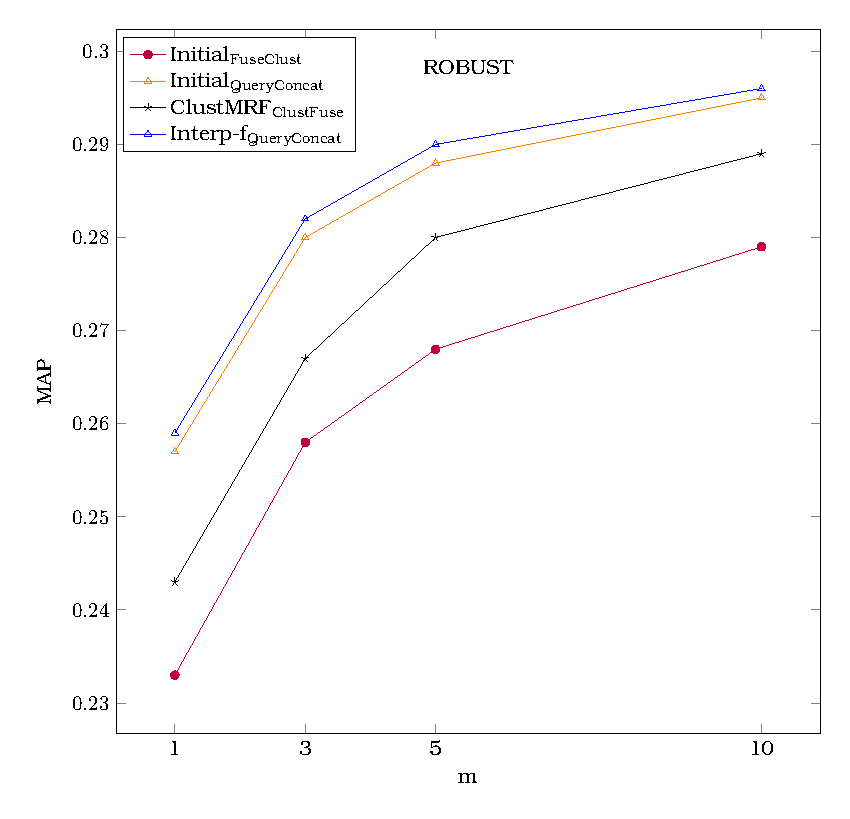
\includegraphics[width=\figWidth, height=\figHeight]{Results2/robust.pdf} &
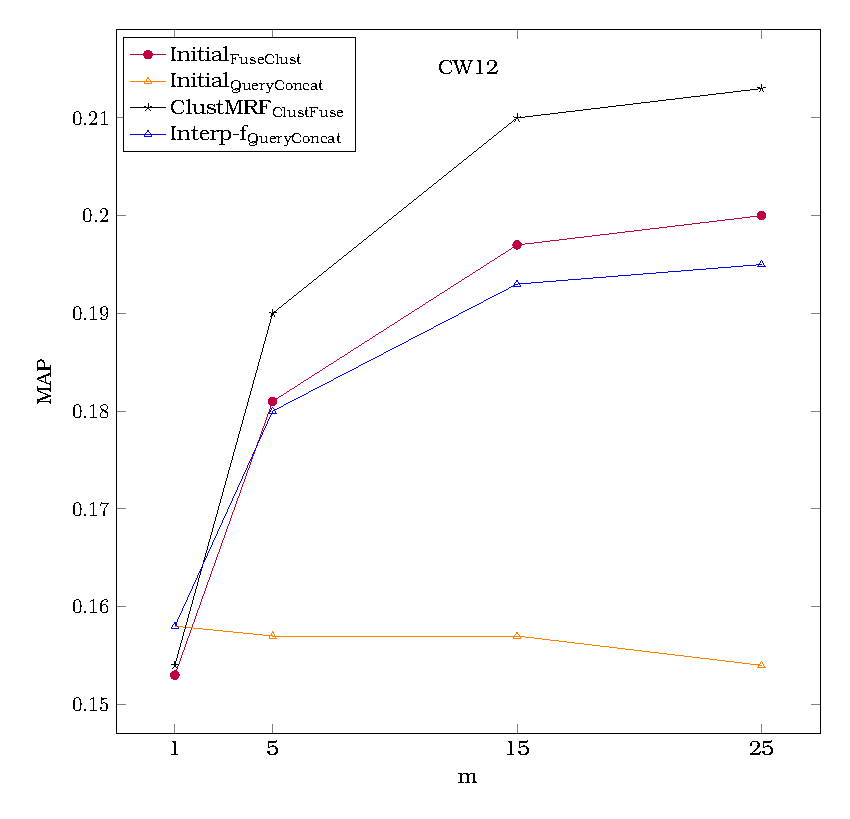
\includegraphics[width=\figWidth, height=\figHeight]{Results2/cw12.pdf}
  \end{tabular}
  \caption{\label{fig:numQuery} The effect on performance of the number of queries used ($\numQuery$) in addition to the \titleQuery query. Note: figures are not to the same scale.}
  \end{figure*}



In Table \ref{tab:compAll} we compare the performance of all methods
instantiated from our templates. As reference comparisons we use the two baselines which were, in general, the most effective among those we considered: the initial document lists used by \fuseClust and \queryCat. (Refer back to Table \ref{tab:main}.) The former is the reciprocal rank fusion of the lists retrieved for the queries, and the latter is standard language-model retrieval with a query which results from concatenating all those available.

We can see in Table \ref{tab:compAll} that \clustFuse and \queryCat
are the two most effective templates across the cluster-based retrieval methods used to instantiate the templates. Indeed, all underlined numbers in the table, which are the best performance per corpus and evaluation measure, appear in rows corresponding to these two templates. Recall that \clustFuse first applies cluster-based retrieval upon each of the lists retrieved for the queries, and then fuses the resultant lists. \queryCat simply concatenates the queries and feeds them to a cluster-based retrieval method. The two best performing methods in the table that are instantiated from these templates are \inst{\interp}{\queryCat} and \inst{\clustMRF}{\clustFuse} which consistently, and almost always statistically significantly, outperform the two baselines.


The least effective template, across the cluster-based methods used
for instantiation, is \poolClust. The second least effective template
is \feature. They are also consistently (and often statistically
significantly) outperformed by the two baselines. Both these templates
leverage the multiple queries at the query-document and/or
query-cluster similarity level; that is, the similarity to a single
query is replaced with the average similarity to all given queries. We
note that the method instantiated from \poolClust using the \interp
cluster retrieval model is a conceptual analog (modulo some technical
details) of a method proposed for cluster-based fusion of document lists
retrieved for a single query by different retrieval systems
\cite{Kozorovitzky+Kurland:11b}.

Additional observation based on Table \ref{tab:compAll} is that the FuseClust template is more effective than \poolClust and \feature and less effective than \clustFuse and \queryCat. The comparison with the first two further attests to the merits of integrating information induced from multiple queries by fusion at the document list level rather than by improving query-similarity estimates. The superiority of ClustFuse to FuseClust means that it is more effective to first re-rank each retrieved least using cluster-based information and then fuse the resultant lists than to first fuse the lists and than utilize cluster-based information from the fused list so as to re-rank it.

We also see in Table \ref{tab:compAll} that the standard single-query
cluster-based retrieval methods (``Title'' rows) are substantially less effective than the templates, including the least performing templates (\poolClust and \feature). This finding further attests to the merits of using multiple queries for retrieval, specifically, with a cluster-based approach.



\subsubsection{The effect of the number of queries}
\label{sec:size}





In Figure \ref{fig:numQuery} we study the effect on performance of the
number of queries, $\numQuery$, in the query set $\querySet$ used in
addition to the \titleQuery query. We present performance numbers for
our two best performing methods, \inst{\interp}{\queryCat} and
\inst{\clustMRF}{\clustFuse}, and the two best performing baselines,
\fuseClust and \queryCat. The baselines are affected by the number of
queries since \fuseClust fuses (using reciprocal rank fusion) the
lists retrieved in response to the queries and \queryCat is standard retrieval in response to the concatenation of all given queries.

We see in Figure \ref{fig:numQuery} that the performance of all
methods, except for \queryCat on CW12, increases with an increased
number of queries. In \queryCat all the queries are concatenated, and
standard language model retrieval applied here is not necessarily very
effective for very long queries \cite{Gupta+Bendersky:15a}.

Figure \ref{fig:numQuery} also shows that for each of the two corpora,
our best performing method almost always consistently outperforms the two baselines; the single exception is $m=1$ for CW12. This finding further attests to the effectiveness of our templates in utilizing information induced from multiple queries, specifically, in a cluster-based document retrieval framework.


%\begin{table}[t]
%\tabcolsep=0.12cm
%\small
%\caption{The cluster hypothesis test. m=5/15, n=50}
%\begin{tabular}{@{}lccccc@{}}
& \queryCat & \fuseClust & \clustFuse & \poolClust & \feature \\
\toprule
\robust &  $.169$ & $.180$&  $.194$ & $\mathbf{.195}$&  $.191$\\
\cw & $.120$ & $.112$&  $.123$ & $\mathbf{.138}$&  $.110$\\
\end{tabular}
%\end{table}

%\begin{table}[t]
%\tabcolsep=0.12cm
%\small
%\caption{Optimal cluster. m=5/15, n=50}
%\begin{tabular}{@{}lccccc@{}}
& \queryCat & \fuseClust & \clustFuse & \poolClust & \feature \\
\toprule
\robust &  $\mathbf{84.1}$ & $83.7$&  $75.9$ & $83.4$&  $77.9$\\
\cw & $82.8$ & $\mathbf{87.4}$&  $74.6$ & $86.6$&  $75.4$\\
\end{tabular}

%\end{table}




